\chapter{Evaluation}
\label{evaluation}

In this chapter, we present and discuss the results of the interview. We evaluate the research questions from the results obtained from the interview. Factors like correctness,time measurements and difficulty ratings help us with the evaluation process. Correctness is presented in \hyperref[sec:4.1]{Section 4.1} and time measurements is presented in \hyperref[sec:4.2]{Section 4.2}. We also present the results of difficult rating in \hyperref[sec:4.3]{Section 4.3}. We then discuss our findings from the results in \hyperref[sec:4.4]{Section 4.4}. We also present certain factors in \hyperref[sec:4.5]{Section 4.5}, that might have influenced our interview unfavourably. Finally, in in \hyperref[sec:4.6]{Section 4.6}, we present feedback given by the interviewees on how the visualization of performance-influence model tool can be improved. 

\section{Correctness}
\label{sec:4.1}
We check the answers given by the interviewees to the questions asked in the questionnaire. We evaluate how often an interviewee answered the question correctly. Evaluation is done with respect to each question and each use case; simple and complex. \hyperref[table:correctness]{Table 4.1} presents the relative number of correct answers given for each use  case with its summary per question. 
 
\begin{table}[!htbp]
\centering
\small
\begin{tabular}{lccccccc}
\toprule   
 Input & Use case & Radar Chart  & Text Plot  & Ratio Plot \\ 
\midrule
& Simple & 100\% &  100\% & 88.8\%\\ 
Q1  & Complex &  100\% &  100\% &  77.7\%\\ 
\midrule
& Summary &  100\% &  100\% &  83.83\%\\
\bottomrule
& Simple & 70\% &  100\% & 60\%\\ 
Q2 & Complex & 100\% & 100\% & NA\\ 
\midrule
& Summary & 83.34\% & 100\% &  60\%\\
\bottomrule
& Simple & 100\% &  100\% & 100\%\\ 
Q3 & Complex & 22.23\% & 100\% & 66.66\%\\ 
\midrule
& Summary & 61.11\% & 100\% &  66.66\%\\
\bottomrule
& Simple & 100\% &  88.89\% & 22.23\%\\ 
Q4 & Complex & 88.89\% & 88.89\% & 55.55\%\\ 
\midrule
& Summary & 94.45\% & 88.89\% &  26.66\%\\
\bottomrule
& Simple &  88.89\% &  88.89\% & 33.34\%\\ 
Q5 & Complex & 33.34\% & 100\% &  88.89\%\\ 
\midrule
& Summary & 77.77\% & 94.44\% &  61.11\%\\
\bottomrule
& Simple &  33.34\% &  22.22\% & 88.88\%\\ 
Q6 & Complex & 55.55\% & 77.77\% &  77.77\%\\ 
\midrule
& Summary & 61.11\% & 50\% & 83.33\%\\
\bottomrule
\end{tabular}
\label{table:correctness}
\caption[Correctness Table]{The relative number of correctly answered questions in the interview for the different visualization techniques
across the different questions and complexities.} 
\end{table}
 
\section{Time Measurements}
\label{sec:4.2}
The second factor to evaluate the research questions, is by taking time measurements.

\begin{table}[!htbp]
\centering
\begin{adjustbox}{width=1\textwidth}
\begin{tabular}{@{\extracolsep{4pt}}lccccccc}
\toprule   
   &  Radar Plot  & Text Plot  & Ratio Plot  & Radar Plot  & Text Plot  & Ratio Plot \\ 
Input & <  & <  & < & > & > & > \\
   &  Text Plot & Ratio Plot & Radar Plot & Text Plot & Ratio Plot & Radar Plot\\
\midrule
Q1 Simple  & 0.535 & 0.638 & 0.5 & 0.5 & 0.395 & 0.535\\ 
Q1 Complex & 0.535 & 0.464 & 0.604 & 0.5 & 0.570 & 0.429\\ 
Q2 Simple  &  0.855 & \textbf{0.010} & 0.953 & 0.165 & 0.991 & \textbf{0.055}\\ 
Q2 Complex & 0.811 & \textbf{--} & \textbf{--} & 0.213 & \textbf{--} & \textbf{--}\\ 
Q3 Simple  & 0.5 & \textbf{0.004} & 0.994 & 0.535 & 0.996 & \textbf{0.006}\\ 
Q3 Complex & 0.982  & \textbf{0.004} & 0.701 & \textbf{0.021} & 0.996 & 0.329\\ 
Q4 Simple & 0.395 & \textbf{0.001} &  0.999 & 0.638 & 0.998 & \textbf{0.000}\\ 
Q4 Complex & 0.638 & \textbf{0.006} & 0.996 & 0.395 & 0.994 &  \textbf{0.004}\\ 
Q5 Simple  & 0.973 & 0.055 & 0.701 & \textbf{0.031} & 0.953 & 0.329\\ 
Q5 Complex & 0.429 & 0.125 & 0.670 & 0.604 & 0.891 & 0.361\\ 
Q6 Simple  & 0.464 & 0.760 & 0.329 & 0.570 & 0.268 & 0.701\\ 
Q6 Complex & 0.535 & 0.188 &  0.811 & 0.5 & 0.834 & 0.213 \\ 
 \midrule
Q1 Simple \& Complex & 0.581 & 0.493 &  0.544 & 0.430 & 0.581 & 0.468\\ 
Q2 Simple \& Complex & 0.920 & \textbf{0.004} &  0.973 & 0.084 & 0.995 &  \textbf{0.030}\\ 
Q3 Simple \& Complex & 0.894 & \textbf{0.000} & 0.976 & 0.111 & 0.999 & \textbf{0.025}\\
Q4 Simple \& Complex & 0.518 & \textbf{0.000} &  0.999 & 0.493 & 0.999 & \textbf{0.000} \\
Q5 Simple \& Complex & 0.899 & \textbf{0.028} & 0.559 & 0.105 & 0.973 &  0.454\\
Q6 Simple \& Complex & 0.455 & 0.369 & 0.665 & 0.556 & 0.642 & 0.346\\
\bottomrule
\end{tabular}
\end{adjustbox}
\label{table:time}
\caption[Mann-Whitney U Test]{Mann-Whitney U test results for the different visualization techniques across the different questions and complexities.} 
\end{table}

Time is measured on how long an interviewee took to answer a question. This is done to compare if an interviewee took longer time to answer a complex use case than a simpler one or to check if one of the visualization techniques was time consuming than the others.

We will conduct the \textit{Mann–Whitney U test} in this section.

\subsection{Mann–Whitney U test}
Mann–Whitney U test helps us to determine, if one sample is significantly better than another sample when time is considered as a factor. We say that the sample is significantly better than another if the p value of the test is less than 0.05. \hyperref[table:time]{Table 4.2}, presents the results for Mann–Whitney U test. The significant values are marked in bold.

In our case, we determine if one group of time measurement is significantly better than another group of time measurement. We compare time measurement groups between radar plot, text plot and ratio plot. 

Here we try to find, if a visualization technique consumed significantly less time than other visualization techniques to answer a question. For instance, radar plot $<$ text plot, implies if radar plot is better than text plot, if the Mann–Whitney U test value is less 0.05. Similarly, radar plot $>$ text plot, implies if radar plot is worse than text plot. 

\section{Difficulty Rating}
\label{sec:4.3}

We also consider difficulty rating as a factor for the evaluation of research questions. Interviewee selects the difficulty rating on how easy or difficult it was to answer a question. This rating corresponds to the time taken by the interviewee to answer the question. \hyperref[table:rating]{Table 4.3}, presents the average difficulty ratings.


\begin{table}[!htbp]
\centering
\small
\begin{tabular}{@{\extracolsep{4pt}}lccccccc}
\toprule   
{} & \textbf{Radar Plot} &   &   \textbf{Text Plot} &   &  \textbf{Ratio Plot}\\
 \cmidrule{2-3} 
 \cmidrule{4-5} 
  \cmidrule{6-7} 
Input  & Mean & & Mean & & Mean \\
\midrule
Q1 Simple  & $1.3\varpm 0.471$ &  & $1.5\varpm 0.496$ &  &   $1.2\varpm 0.415$& \\ 
Q1 Complex & $2.4\varpm 0.831$ &  & $2.2\varpm 0.628$ &  &   $1.3\varpm 0.471$& \\ 
Q2 Simple  & $1.5\varpm 0.684$ &  & $1.5\varpm 0.831$ &  &   $4.2\varpm 1.030$& \\ 
Q2 Complex & $1.8\varpm 0.566$ &  & $2\varpm 0.471$ &  & \textbf{--} & \\ 
Q3 Simple  & $1.5\varpm 0.496$ &  & $1.6\varpm 0.666$ &  &   $3.1\varpm 1.286$& \\ 
Q3 Complex & $2.8\varpm 1.099$ &  & $2.1\varpm 0.314$ &  &   $3.4\varpm 1.065$& \\ 
Q4 Simple  & $1.6\varpm 0.471$ &  & $1.7\varpm 0.415$ &  &   $3.7\varpm 0.916$& \\ 
Q4 Complex & $2.4\varpm 0.496$ &  & $1.8\varpm 0.314$ &  &   $3.5\varpm 0.955$& \\  
Q5 Simple  & $2.6\varpm 1.054$ &  & $2.2\varpm 0.785$ &  &   $4.3\varpm 0.942$& \\  
Q5 Complex & $2.8\varpm 0.993$ &  & $1.7\varpm 0.628$ &  &   $4.4\varpm 0.684$& \\ 
Q6 Simple  & $2.7\varpm 0.628$ &  & $3\varpm 0.666$ &  &   $3.6\varpm 1.054$& \\ 
Q6 Complex & $2.3\varpm 0.471$ &  & $2.5\varpm 0.955$ &  &   $4.2\varpm 1.030$& \\ 
 \midrule
Q1 Simple \& Complex  & $1.8\varpm 0.874$ &  & $1.8\varpm 0.657$ &  &   $1.2\varpm 0.447$& \\ 
Q2 Simple \& Complex  & $1.7\varpm 0.650$ &  & $1.7\varpm 0.711$ &  &   $4.2\varpm 1.030$& \\ 
Q3 Simple \& Complex  & $2.2\varpm 1.082$ &  & $1.8\varpm 0.566$ &  &   $3.2\varpm 1.192$& \\ 
Q4 Simple \& Complex  & $2.0\varpm 0.621$ &  & $1.8\varpm 0.372$ &  &   $3.6\varpm 0.942$& \\
Q5 Simple \& Complex  & $2.7\varpm 1.030$ &  & $2\varpm 0.745$ &  &   $4.3\varpm 0.825$& \\
Q6 Simple \& Complex  & $2.5\varpm 0.598$ &  & $2.7\varpm 0.853$ &  &   $3.9\varpm 1.078$& \\ 
\bottomrule
\end{tabular}
\label{table:rating}
\caption[Difficulty Rating]{Average difficulty rating for the different visualization techniques across the different questions and complexities.} 
\end{table}

\subsection{Pearson's correlation Test}
We conduct Pearson's correlation test with difficulty ratings and time measurements as input. This test helps to determine the measure of linear correlation between the 2 inputs. The inputs we use for this test are the time measurements and difficulty ratings for different visualization techniques and different questions along with their complexities. \hyperref[table:pearons]{Table 4.4}, presents the linear correlation values for the same.

The p values range from -1 to +1. A values less than 0.5 implies weak correlation, value between 0.5 - 0.8 implies medium correlation and value greater than 0.8 implies strong correlation. A positive p value implies that both inputs increase or decrease linearly and a negative p value implies that both increase or decrease inversely.

\begin{table}[!htbp]
\centering
\begin{tabular}{@{\extracolsep{4pt}}lccccccc}
\toprule   
{} & \textbf{Radar Plot} &   &   \textbf{Text Plot} &   &  \textbf{Ratio Plot}\\
 \cmidrule{2-3} 
 \cmidrule{4-5} 
  \cmidrule{6-7} 
Input  & p value &  & p value &  & p value \\
\midrule
Q1 Simple  & -0.013 &  & 0.216 &  & 0.711 & \\ 
Q1 Complex & 0.637 &  & 0.403 &  & -0-218 & \\ 
Q2 Simple  & 0.384 &  & -0.280 &  & -0.019 & \\ 
Q2 Complex & 0.753 &  & 0.576 &  & \textbf{--} & \\ 
Q3 Simple  & 0.877 &  & 0.566 &  & 0.506 & \\ 
Q3 Complex & 0.163 &  & 0.509 &  & 0.119 & \\ 
Q4 Simple  & 0.350 &  & 0.347 &  & 0.626 &\\ 
Q4 Complex & -0.268 &  & 0.373 &  & -0.280 &\\ 
Q5 Simple  & 0.289 &  & 0.493 &  & 0.401 &\\ 
Q5 Complex & 0.618 &  & 0.773 &  & -0.133 &\\ 
Q6 Simple  & -0.145 &  & -0.268  &  & 0.519 &\\ 
Q6 Complex & 0.293 &  & 0.178  &  & 0.487 &\\ 
\bottomrule
\end{tabular}
\label{table:pearons}
\caption[Difficulty Rating]{Pearson's Test for the different visualization techniques across the different questions and complexities.} 
\end{table}

Time measurements and difficulty ratings are also plotted for each interviewee, for each question. This is done so as to look at the correlation between them graphically. These plots are presented in \hyperref[sanityCheck]{Appendix:A.1}

\section{Results}
\label{sec:4.4}

We now answer the research questions by using the results from the correctness values, the time measurements, and the difficulty ratings.

We also use pareto-front plots for each research question. So far we have seen the two evaluation factors; correctness and time separately. Using pareto-front plots, we combine these two factors. These plots are plotted with time vs correctness. They help us to determine which visualization technique is the best when considering both these evaluation factors. A visualization is considered best when it takes lowest amount of time to answer a question with highest relative number of correct values.

\subsection*{One Performance-Influence Model}
\vskip 0.2in
\begin{mdframed}
\textbf{RQ1: Can we use the visualization techniques to identify relevant configuration options or interactions  of one performance-influence model?}
\end{mdframed}

We consider Q1 and Q2 for this research question.

\begin{description}[leftmargin=0pt]
\item[Correctness: ]From \hyperref[table:correctness]{Table 4.1}, we can see that all the interviewees were able to answer both Q1 and Q2 correctly when presented with radar plot and text plot, regardless of the use case. With ratio plot there are chances that a user might not get the intended answer. We can infer, that the relative number of in correct answers given to ratio plot is not high, but we might not always get the correct answer. 
  
\item[Time Measurements: ]From the results presented in \hyperref[table:time]{Table 4.2} for Q1 and Q2, we see that there is no significant time differences between the visualization techniques for Q1 for both the use cases. However, for Q2, we see that for the simple use case text plot performed significantly better than other visualization techniques.
  
\item[Difficulty Ratings: ]From the difficulty ratings presented in \hyperref[table:rating]{Table 4.3}, we can note that the average difficulty ratings for Q1 and Q2 are below 2.4 with an exception of ratio plot for Q2, for the simple use case. Where it has an average rating of 4.2, but also with a higher standard deviation.

\end{description}

Hence, the answer to this research question would be \textbf{yes}, with text plot being the considerable choice of visualization, since it has best results when considering both time and correctness factors.

\vskip 0.2in
\begin{mdframed}
\textbf{RQ1.1: Can we use the visualization techniques to identify relevant configuration options or interactions  of one simple performance-influence model?}
\end{mdframed}

\textbf{Q1}: From \hyperref[figure:paretoOneQ1]{Figure 4.1}, for the simple use case text plot is much better than other visualization techniques. We can also notice that ratio plot takes slightly less time, but does not guarantee perfect correctness results.

\textbf{Q2}: From \hyperref[figure:paretoOneQ2]{Figure 4.2}, for the simple use case text plot is much better both in terms of time and correctness. 

\begin{figure}[hbt!]
\centering
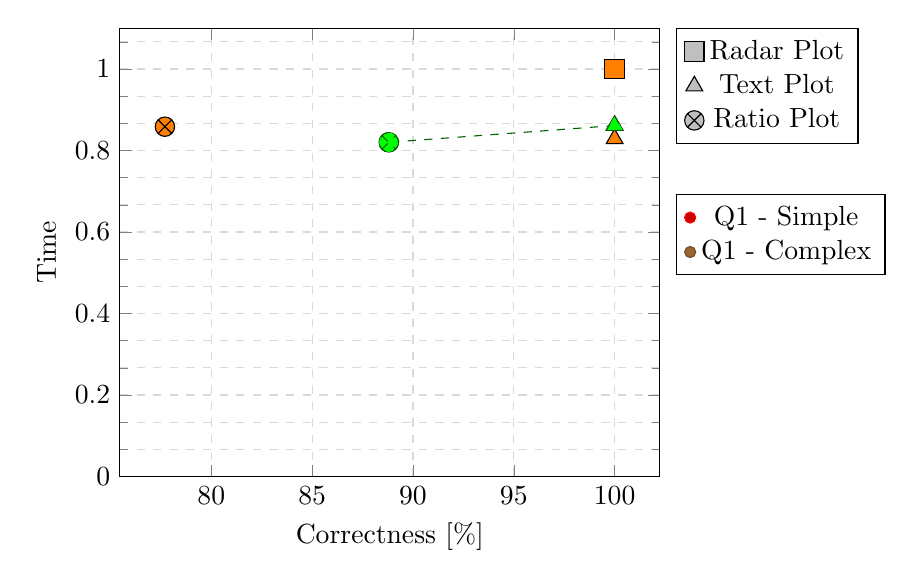
\begin{tikzpicture}
\definecolor{clr1}{RGB}{0,100,0}
\definecolor{clr2}{RGB}{255,165,0}
	\begin{axis}[%
	xlabel={Correctness [\%]},
    ylabel={Time},
    ymin=0,
    minor y tick num=2,
    grid style={dashed,gray!30},
    ymajorgrids=true,
    xmajorgrids=true,
    yminorgrids=true,
    only marks,
    scatter,
    mark size=3.5pt,
    scatter src=explicit symbolic,
	scatter/classes={
		x={mark=square*,fill=lightgray},
		y={mark=triangle*,fill=lightgray},
		z={mark=otimes*,fill=lightgray},
		a={mark=square*,fill=green},
		b={mark=triangle*,fill=green},
		c={mark=otimes*,fill=green},
		d={mark=square*,fill=orange},
		e={mark=triangle*,fill=orange},
		f={mark=otimes*,fill=orange}},
	     legend entries={
            Radar Plot,
            Text Plot,
            Ratio Plot%
        },
        legend pos=outer north east,]
	\addplot[scatter,only marks,%
		scatter src=explicit symbolic]%
	table[meta=label] {
x         y         label
100       1         a  
100       0.8612    b 
88.8      0.8201    c 
100       1         d 
100       0.8288    e 
77.7      0.8584    f 
};
\addplot +[clr1, smooth, dashed] table[meta=label]  {
x          y         label 
100       0.8612      b 
88.8      0.8201      c 
}; 
\end{axis}
	
\begin{axis}[
    xmin=0,
    xmax=100,
    ymin=1,
    ymax=6,
    hide axis,
    only marks,
    legend entries={
     ,       % the dummy plot should not show up in the legend
        Q1 - Simple,
        Q1 - Complex,%  
    },
     legend pos=outer north east,
    legend style={
            yshift=-60pt,
        },
    ]
\foreach \i in {0,...,6} {
        \addplot+ [mark=*] coordinates { (0,0) };
     }
    \end{axis}
\end{tikzpicture}
\label{figure:paretoOneQ1}
\caption[Pareto-front for Q1]{The correctness and time values for Q1 (simple and complex). The pareto front for the different complexities is drawn by using a green and orange line respectively. The visualizations on the pareto front for Q1 - Simple is text and ratio plot and for Q1 - Complex is the text plot.} 
\end{figure}

\begin{figure}[hbt!]
\centering
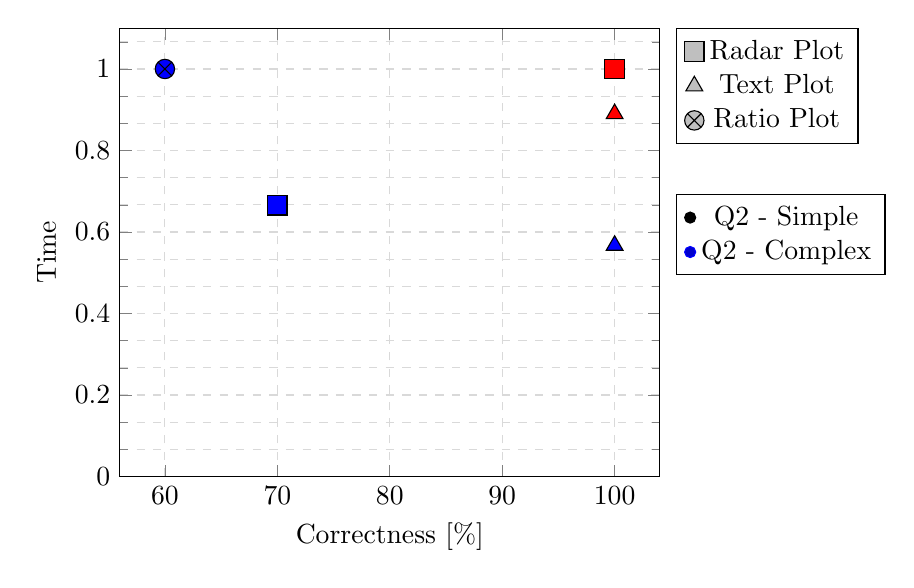
\begin{tikzpicture}
	\begin{axis}[%
	xlabel={Correctness [\%]},
    ylabel={Time},
    ymin=0,
    minor y tick num=2,
    grid style={dashed,gray!30},
    ymajorgrids=true,
    xmajorgrids=true,
    yminorgrids=true,
    only marks,
    scatter,
    mark size=3.5pt,
    scatter src=explicit symbolic,
	scatter/classes={
		x={mark=square*,fill=lightgray},
		y={mark=triangle*,fill=lightgray},
		z={mark=otimes*,fill=lightgray},
		g={mark=square*,fill=blue},
	    h={mark=triangle*,fill=blue},
		i={mark=otimes*,fill=blue},
		j={mark=square*,fill=red},
	    k={mark=triangle*,fill=red}},
	     legend entries={
            Radar Plot,
            Text Plot,
            Ratio Plot%
        },
        legend pos=outer north east,]
	\addplot[scatter,only marks,%
		scatter src=explicit symbolic]%
	table[meta=label] {
x         y         label
70        0.6656    g  
100       0.567     h 
60        1         i 
100       1         j 
100       0.89      k 
};
\end{axis}
	
\begin{axis}[
    xmin=0,
    xmax=100,
    ymin=1,
    ymax=6,
    hide axis,
    only marks,
    legend entries={
     ,   ,  ,  % the dummy plot should not show up in the legend
        Q2 - Simple,
        Q2 - Complex%
    },
     legend pos=outer north east,
    legend style={
            yshift=-60pt,
        },
    ]
\foreach \i in {0,...,6} {
        \addplot+ [mark=*] coordinates { (0,0) };
     }
    \end{axis}
\end{tikzpicture}
\label{figure:paretoOneQ2}
\caption[Pareto-front for Q2]{The correctness and time values for Q2 (simple and complex). The pareto front for the different complexities is drawn by using a blue and red line respectively. The visualizations on the pareto front for Q2 - Simple is text plot and for Q2 - Complex is the text plot.} 
\end{figure}

\vskip 0.2in
\begin{mdframed}
\textbf{RQ1.2: Can we use the visualization techniques to identify relevant configuration options or interactions  of one complex performance-influence model?}
\end{mdframed}

\textbf{Q1}: From \hyperref[figure:paretoOneQ1]{Figure 4.1}, we can notice that for the complex use case, both radar plot and text plot perform equally better in terms of correctness, however text plot performed slightly better in terms of time. Whereas, ratio plot did not perform as good as text and radar plot.

\textbf{Q2}: From \hyperref[figure:paretoOneQ2]{Figure 4.2}, for the complex use case, text plot is slightly better than radar plot both in terms of time and correctness. Ratio plot was not considered for this question, since ratio plot displays the general influence of a configuration option or interaction, also that the ratio plot does not display configuration options with zero or no influence.

In the complex use case too text plot is better, for the same reasons as mentioned in the previous research question.

Hence, to answer all the above research questions, we can say that \textbf{yes}, we can use visualization techniques to identify relevant properties of one performance-influence model.

\subsection*{Two Performance-Influence Models}
\vskip 0.2in
\begin{mdframed}
\textbf{RQ2: Can we use the visualization to compare two performance-influence models?}
\end{mdframed}

We consider Q3 and Q4 for this research question.

\begin{description}[leftmargin=0pt]
\item[Correctness: ]From \hyperref[table:correctness]{Table 4.1}, we can see that all the interviewees were able to answer Q3 correctly for all the visualization techniques, for the simple use case. However, for the complex use case, only text plot performed well. For Q4, radar plot performed comparatively better than other visualization techniques for both the use case.

\item[Time Measurements: ]From the results presented in \hyperref[table:time]{Table 4.2}, we see that for both Q3 and Q4, text plot is significantly better than other visualization techniques regardless of the use case of the questions. It implies that text plot took significantly less time to answer the questions.

\item[Difficulty Ratings: ] From \hyperref[table:rating]{Table 4.3}, for Q3 and Q4 and for both the use case, we notice that ratio plot stands out as it has consistently higher difficulty ratings than radar and text plot. 
\end{description}

Hence, the answer to this research question would be \textbf{yes}, with text plot being the considerable choice of visualization technique, since it has best results when considering both time and correctness factors.

The reason being that two performance-influence models are easier and faster to compare when they are visualized side-by-side as in text plot. When they are visualized in ratio plot, the same configuration option or interaction are not plotted side-by-side, their order differ based on their general performance. Hence, comparison on text plot is easier than on ratio plot. 

Radar plot does moderately good at comparison, since data is plotted in a circle than in a textual order.

\vskip 0.2in
\begin{mdframed}
\textbf{RQ2.1: Can we use the visualization to compare two simple performance-influence models?}
\end{mdframed}

\textbf{Q3:} From \hyperref[figure:paretoTwoQ3]{Figure 4.3}, for the simple use case, we can infer that both text plot and radar plot are equally better, when both factors; correctness and time are considered. We also see that both these visualization techniques produce perfect correctness results.

\textbf{Q4:} From \hyperref[figure:paretoTwoQ4]{Figure 4.4}, for the simple use case, radar plot is better in terms of correctness measurements. But, from \hyperref[table:time]{Table 4.2}, we know text plot does significantly better than other visualization techniques. This implies that even though interviewees took less time to answer text plot, the results were not 100\% correct.

We can also see both the ratio plots marking are at the very top, indicating that they take highest time to answer the question, which did not always lead to correct answers.

\begin{figure}[hbt!]
\centering
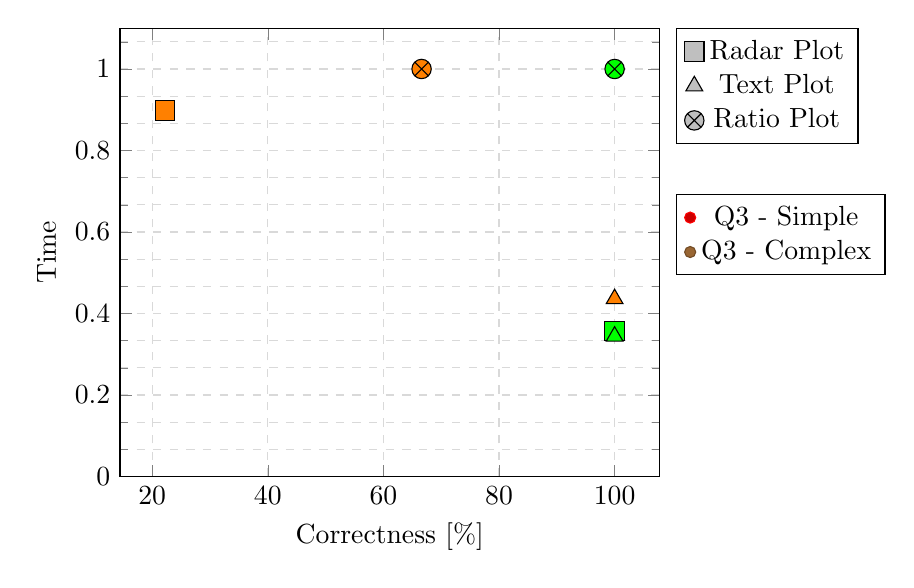
\begin{tikzpicture}
	\begin{axis}[%
	xlabel={Correctness [\%]},
    ylabel={Time},
    ymin=0,
    minor y tick num=2,
    grid style={dashed,gray!30},
    ymajorgrids=true,
    xmajorgrids=true,
    yminorgrids=true,
    only marks,
    scatter,
    mark size=3.5pt,
    scatter src=explicit symbolic,
	scatter/classes={%
		x={mark=square*,fill=lightgray},
		y={mark=triangle*,fill=lightgray},
		z={mark=otimes*,fill=lightgray},
		a={mark=square*,fill=green},%
		b={mark=triangle*,fill=green},%
		c={mark=otimes*,fill=green},%
		d={mark=square*,fill=orange},%
		e={mark=triangle*,fill=orange},%
		f={mark=otimes*,fill=orange}},
	     legend entries={
            Radar Plot,
            Text Plot,
            Ratio Plot%
        },
        legend pos=outer north east,]]
	\addplot[scatter,only marks,%
		scatter src=explicit symbolic]%
	table[meta=label] {
x         y            label
100       0.357        a  
100       0.344        b 
100       1            c 
22.20     0.898        d 
100       0.436        e 
66.6      1            f 
	};
	
\end{axis}

\begin{axis}[
    xmin=0,
    xmax=100,
    ymin=1,
    ymax=6,
    hide axis,
    only marks,
    legend entries={
     ,       % the dummy plot should not show up in the legend
        Q3 - Simple,
        Q3 - Complex,%
    },
     legend pos=outer north east,
    legend style={
            yshift=-60pt,
        },
    ]
\foreach \i in {0,...,6} {
        \addplot+ [mark=*] coordinates { (0,0) };
     }
    \end{axis}
\end{tikzpicture}
\label{figure:paretoTwoQ3}
\caption[Pareto-front for Q3]{The correctness and time values for Q3 (simple and complex). The pareto front for the different complexities is drawn  by using a green and orange line respectively. The visualizations on the pareto front for Q3 - Simple is radar and text plot and for Q3 - Complex is the text plot.} 
\end{figure}

\begin{figure}[hbt!]
\centering
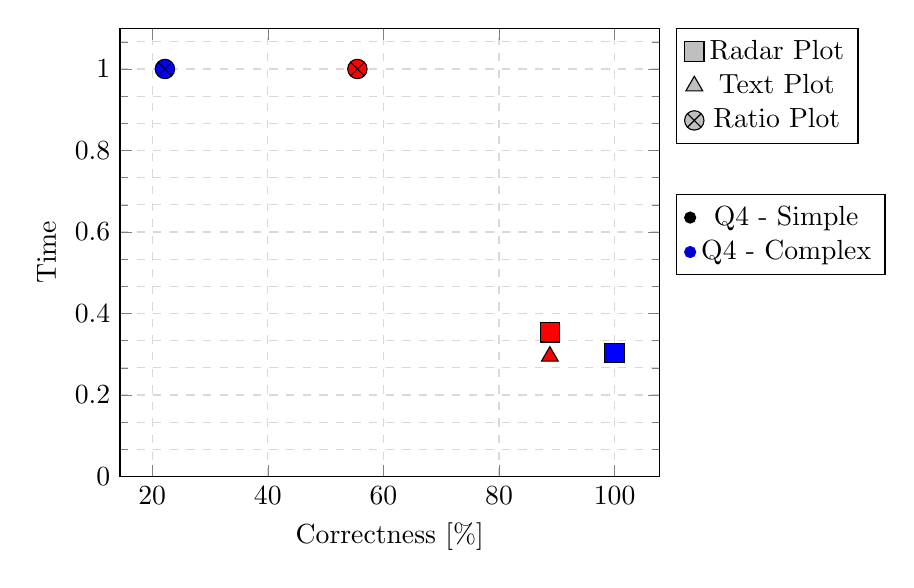
\begin{tikzpicture}
	\begin{axis}[%
	xlabel={Correctness [\%]},
    ylabel={Time},
    ymin=0,
    minor y tick num=2,
    grid style={dashed,gray!30},
    ymajorgrids=true,
    xmajorgrids=true,
    yminorgrids=true,
    only marks,
    scatter,
    mark size=3.5pt,
    scatter src=explicit symbolic,
	scatter/classes={%
		x={mark=square*,fill=lightgray},
		y={mark=triangle*,fill=lightgray},
		z={mark=otimes*,fill=lightgray},
		g={mark=square*,fill=blue},%
	    h={mark=triangle*,fill=blue},%
		i={mark=otimes*,fill=blue},%
		j={mark=square*,fill=red},%
	    k={mark=triangle*,fill=red},%
	    l={mark=otimes*,fill=red}},
	     legend entries={
            Radar Plot,
            Text Plot,
            Ratio Plot%
        },
        legend pos=outer north east,]]
	\addplot[scatter,only marks,%
		scatter src=explicit symbolic]%
	table[meta=label] {
x         y            label
100       0.303        g  
88.80     0.354        h 
22.20     1            i 
88.80     0.354        j 
88.80     0.295        k 
55.50     1            l 
	};

\end{axis}

\begin{axis}[
    xmin=0,
    xmax=100,
    ymin=1,
    ymax=6,
    hide axis,
    only marks,
    legend entries={
     ,   , ,    % the dummy plot should not show up in the legend
        Q4 - Simple,
        Q4 - Complex%
    },
     legend pos=outer north east,
    legend style={
            yshift=-60pt,
        },
    ]
\foreach \i in {0,...,6} {
        \addplot+ [mark=*] coordinates { (0,0) };
     }
    \end{axis}
\end{tikzpicture}
\label{figure:paretoTwoQ4}
\caption[Pareto-front for Q4]{The correctness and time values for Q4 (simple and complex). The pareto front for the different complexities is drawn by using a blue and red line respectively. The visualizations on the pareto front for Q4 - Simple is radar plot and for Q4 - Complex is the text plot.}
\end{figure}

\vskip 0.2in
\begin{mdframed}
\textbf{RQ2.2: Can we use the visualization to compare two complex performance-influence models?}
\end{mdframed}

\textbf{Q3:} From \hyperref[figure:paretoTwoQ3]{Figure 4.3}, for the complex use case, we can infer that both text plot outperformed other visualization techniques, when both factors; correctness and time are considered.

\textbf{Q4:} From \hyperref[figure:paretoTwoQ4]{Figure 4.4}, for the complex use case, we can infer that text plot is slightly better than radar plot both in terms of time and correctness factors, even though it did not lead to perfect correctness results.

Text plot is better since comparison of performances in a textual way, is much easier and faster than on radar and ratio plots.

Hence, the answer to all the above research questions would be \textbf{yes}, we can compare two performance-influence models with text plot being the choice of visualization.

\subsection*{Many Performance-Influence Models}

\vskip 0.2in
\begin{mdframed}
\textbf{RQ3: How good can the visualizations be used to compare a high number of performance-influence models and a high number of terms?}
\end{mdframed}

We consider Q5 and Q6 for this research question.

Q5 corresponds to scalability with respect to addition of performance-influence models and Q6 corresponds to scalability with respect to addition of configuration option or interactions.

\begin{description}[leftmargin=0pt]
\item[Correctness: ]From \hyperref[table:correctness]{Table 4.1}, we can see for Q5, we see that text plot is better and for Q6 ratio plot is better to answer this question.

\item[Time Measurements: ]From the results presented in \hyperref[table:time]{Table 4.2} for Q5 and Q6, we see that for both the question there is no significant time differences between the visualization techniques, but from Q5 simple, we can infer that interviewees took significantly longer time to answer question based on radar plot than on text plot.

\item[Difficulty Ratings: ]The difficulty ratings for Q5 and Q6 in \hyperref[table:rating]{Table 4.3}, ratio plot has higher difficulty ratings that other radar and text plot. We have already seen that ratio plot has relative number of correct answers for Q6. This implies that even though ratio plot has a higher difficulty rating, it helps the users get the intended answer.
\end{description}

Therefore, the answer to this research question would be \textbf{yes}, with text plot being the considerable choice of visualization technique, when scalability with respect to performance-influence models is considered, since it has best results when considering both time and correctness factors.

And when scalability with respect to configuration options is considered, ratio plot is the best visualization technique in general.

We already know than for comparing several performance-influence models, text plot is best choice of visualization, since data is easier and also faster to perceive when displayed in a textual way.

For comparing many configuration options among several performance-influence model, ratio plot proved to be better than text and radar plot. The reason can be that when many terms are introduced, the visualization for radar and text can get quite complex and hard to read and compare. Whereas, for ratio plot the bars are spread out, helping the user to do comparisons. The comparisons using ratio plot can be time consuming, but they lead to highest correct answers than the other two visualizations.

\begin{mdframed} 
\textbf{RQ3.1: How good can the visualizations be used to compare a high number of simple performance-influence models and a high number of terms?}
\end{mdframed}

\textbf{Q5:} From \hyperref[figure:paretoManyQ5]{Figure 4.5}, for the simple use case, we can see that text plot is better choice of visualization technique when considering both time and correctness factors.

\textbf{Q6:} From \hyperref[figure:paretoManyQ6]{Figure 4.6}, for the simple use case, we can infer that if time is considered as a factor, radar plot performs comparatively better than other visualization techniques. However, when correctness is considered as a factor, ratio plot performs better. Even though both these plots do not lead to perfect correctness results.

\begin{figure}[hbt!]
\centering
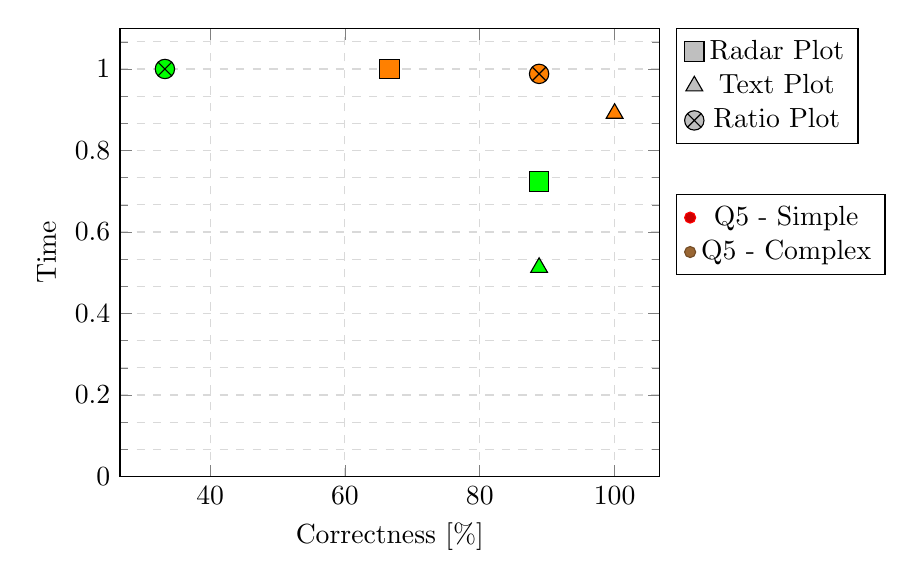
\begin{tikzpicture}
	\begin{axis}[%
	xlabel={Correctness [\%]},
    ylabel={Time},
    ymin=0,
    minor y tick num=2,
    grid style={dashed,gray!30},
    ymajorgrids=true,
    xmajorgrids=true,
    yminorgrids=true,
    only marks,
    scatter,
    mark size=3.5pt,
    scatter src=explicit symbolic,
	scatter/classes={%
		x={mark=square*,fill=lightgray},
		y={mark=triangle*,fill=lightgray},
		z={mark=otimes*,fill=lightgray},
		a={mark=square*,fill=green},%
		b={mark=triangle*,fill=green},%
		c={mark=otimes*,fill=green},%
		d={mark=square*,fill=orange},%
		e={mark=triangle*,fill=orange},%
		f={mark=otimes*,fill=orange}},
	     legend entries={
            Radar Plot,
            Text Plot,
            Ratio Plot%
        },
        legend pos=outer north east,]]
	\addplot[scatter,only marks,%
		scatter src=explicit symbolic]%
	table[meta=label] {
x         y            label
88.80     0.724        a  
88.80     0.513        b 
33.30     1            c 
66.60     1            d 
100       0.891        e 
88.80     0.988        f 
	};
	\end{axis}
\begin{axis}[
    xmin=1,
    xmax=100,
    ymin=1,
    ymax=6,
    hide axis,
    only marks,
    legend entries={
     ,       % the dummy plot should not show up in the legend
        Q5 - Simple,
        Q5 - Complex%
    },
     legend pos=outer north east,
    legend style={
            yshift=-60pt,
        },
    ]
\foreach \i in {0,...,6} {
        \addplot+ [mark=*] coordinates { (0,0) };
     }
    \end{axis}
\end{tikzpicture}
\label{figure:paretoManyQ5}
\caption[Pareto-front for Q5]{The correctness and time values for Q5 (simple and complex). The pareto front for the different complexities is drawn by using a green and orange line respectively. The visualizations on the pareto front for Q5 - Simple is text plot and for Q5 - Complex is the text plot.} 
\end{figure}

\begin{figure}[hbt!]
\centering
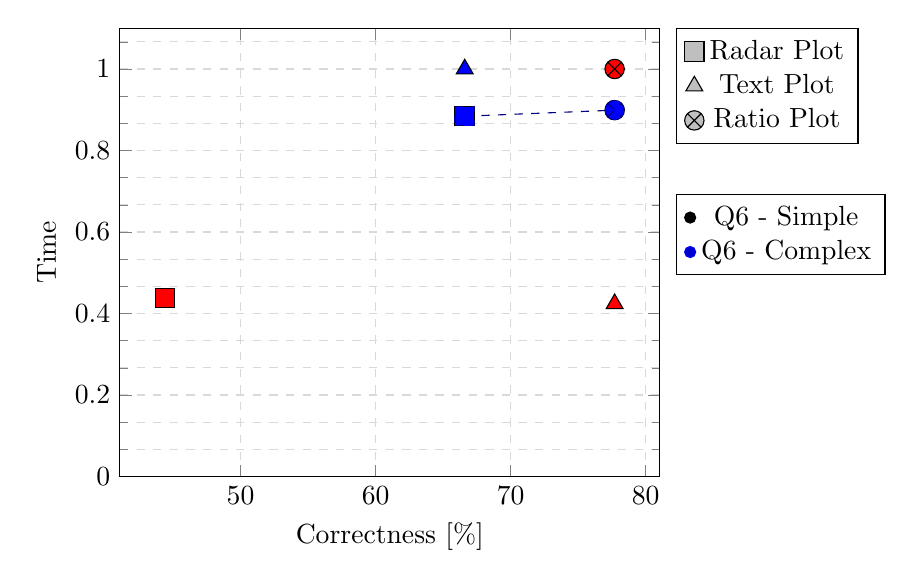
\begin{tikzpicture}
\definecolor{clr1}{RGB}{139,0,0}    
\definecolor{clr2}{RGB}{0,0,128} 
	\begin{axis}[%
	xlabel={Correctness [\%]},
    ylabel={Time},
    ymin=0,
    minor y tick num=2,
    grid style={dashed,gray!30},
    ymajorgrids=true,
    xmajorgrids=true,
    yminorgrids=true,
    only marks,
    scatter,
    mark size=3.5pt,
    scatter src=explicit symbolic,
	scatter/classes={%
		x={mark=square*,fill=lightgray},
		y={mark=triangle*,fill=lightgray},
		z={mark=otimes*,fill=lightgray},
		g={mark=square*,fill=blue},%
	    h={mark=triangle*,fill=blue},%
		i={mark=otimes*,fill=blue},%
		j={mark=square*,fill=red},%
	    k={mark=triangle*,fill=red},%
	    l={mark=otimes*,fill=red}},
	     legend entries={
            Radar Plot,
            Text Plot,
            Ratio Plot%
        },
        legend pos=outer north east,]]
	\addplot[scatter,only marks,%
		scatter src=explicit symbolic]%
	table[meta=label] {
x         y            label
66.60     0.884        g  
66.60     1            h 
77.70     0.899        i 
44.40     0.438        j 
77.70     0.424        k 
77.70     1            l 
	};
\addplot +[clr2, smooth, dashed] table[meta=label]  {
x          y         label 
66.60     0.884        g  
77.70     0.899        i 
}; 	
	\end{axis}
\begin{axis}[
    xmin=0,
    xmax=100,
    ymin=1,
    ymax=6,
    hide axis,
    only marks,
    legend entries={
     ,  ,  ,     % the dummy plot should not show up in the legend
        Q6 - Simple,
        Q6 - Complex%
    },
     legend pos=outer north east,
    legend style={
            yshift=-60pt,
        },
    ]
\foreach \i in {0,...,6} {
        \addplot+ [mark=*] coordinates { (0,0) };
     }
    \end{axis}
\end{tikzpicture}
\label{figure:paretoManyQ6}
\caption[Pareto-front for Q6]{The correctness and time values for Q6 (simple and complex). The pareto front for the different complexities is drawn by  using a blue and red line respectively. The visualizations on the pareto front for Q6 - Simple is radar and ratio plot and for Q6 - Complex is the text plot.} 
\end{figure}
 
\begin{mdframed} 
\textbf{RQ3.2: How good can the visualizations be used to compare a high number of complex performance-influence models and a high number of terms?}
\end{mdframed}

\textbf{Q5:} From \hyperref[figure:paretoManyQ5]{Figure 4.5}, for the complex use case, we can see that if both time and correctness factors are considered text plot performs better than other visualization technique, with perfect correctness measurements.

\textbf{Q6:} From \hyperref[figure:paretoManyQ6]{Figure 4.6}, for the complex use case, we can infer that text plot performs considerably better than ratio plot in terms of time measurements, and better than radar plot in terms of correctness measurements.

\vskip 0.2in
\begin{mdframed}
\textbf {RQ4: What are the differences with respect to visualization techniques regarding many performance-influence models?}
\end{mdframed}

For the above research question and its sub-questions, we use Mann-Whitney test results and box-plot visualizations. 

\begin{description}[leftmargin=0pt]
\item[Mann-Whitney U Test: ]For this test, we use the difficulty ratings for each visualization technique and for each use case. For instance, for Q5 and radar plot the inputs are the difficulty ratings of radar plot for simple use case and radar plot for complex use case of Q5.

\begin{table}[!htbp]
\centering
\begin{tabular}{@{\extracolsep{4pt}}lccccccc}
\toprule   
Input & &\textbf{Radar Plot} &   &   \textbf{Text Plot} &   &  \textbf{Ratio Plot}\\
\midrule
Q5   &   &  0.274 &  & 0.887  & & 0.5\\ 
Q6   &   &  0.938 &  &   0.947 &  & 0.151  \\ 
\bottomrule
\end{tabular}
\label{table:q5q6MannWhitney}
\caption[Difficulty Rating]{Mann-Whitney U Test for the different visualization techniques and complexities for Q5 and Q6.} 
\end{table}

\item[Box Plots: ] The box plot have the co-ordinates time vs simple, complex use cases per visualization type. For instance, for radar plot, we calculate the average time taken per question, when presented with a radar plot with a simple use case and similarly for the complex use case.

\begin{minipage}[b]{0.5\textwidth}
\centering
\begin{tikzpicture}[scale=0.85]
  \begin{axis}
    [ylabel =
        {Time(in seconds)},
    boxplot/draw direction=y,
    xtick={1,2},
    ymin=0,
    minor y tick num=4,
    xticklabels={Simple, Complex, Both},
    x tick label style={font=\footnotesize, text width=2cm, align=center}
    ]
    \addplot+[line width=1pt,mark = *, mark options = {red},
    boxplot prepared={
      lower whisker=17.963,
      lower quartile=44.865,
      median=63.705,
      upper quartile=85.7025,
      upper whisker=125.0
    }, color = red
    ] coordinates{};
    \addplot+[line width=1pt,mark = *,mark options = {blue},
    boxplot prepared={
      lower whisker=13.229,
      lower quartile= 21.3095,
      median= 31.425,
      upper quartile=56.053,
      upper whisker=74.4
    }, color = blue
    ] coordinates{};
     \addplot[ultra thick, color=blue,mark=*] coordinates {
		(2,171.4)
    };
    \addplot[ultra thick, color=blue,mark=*] coordinates {
		(2,122.44)
    };
    \end{axis}
\end{tikzpicture}
\label{scalabilityRadar}
\captionof{figure}{Scalability of radar plot}
\end{minipage}
\begin{minipage}[b]{0.5\textwidth}
\centering
\begin{tikzpicture}[scale=0.85] 
  \begin{axis}
    [ylabel =
       {Time(in seconds)},
    boxplot/draw direction=y,
    xtick={1,2},
    xticklabels={Simple, Complex},
    ymin=0,
    minor y tick num=4,
    x tick label style={font=\footnotesize, text width=2cm, align=center}
    ]
    \addplot+[line width=1pt,mark = *, mark options = {red},
    boxplot prepared={
     lower whisker=25.58,
      lower quartile=32.6465,
      median= 40.7475,
      upper quartile=74.335,
      upper whisker=132.190
    }, color = red
    ] coordinates{};
    \addplot+[line width=1pt,mark = *,mark options = {blue},
    boxplot prepared={
      lower whisker=17.255,
      lower quartile=24.8825,
      median= 34.205,
      upper quartile=54.507,
      upper whisker=65.0
    }, color = blue
    ] coordinates{};
    \addplot[ultra thick, color=blue,mark=*] coordinates {
		(2,197.0)
    };
    \end{axis}
\end{tikzpicture}
\label{scalabilityText}
\captionof{figure}{Scalability of text plot}
\end{minipage}
\begin{center}
\begin{tikzpicture}[scale=0.85] 
  \begin{axis}
    [ylabel ={Time(in seconds)},
    boxplot/draw direction=y,
    xtick={1,2},
    xticklabels={Simple, Complex, Both},
    ymin=0,
    minor y tick num=4,
    x tick label style={font=\footnotesize, text width=2cm, align=center}
    ]
    \addplot+[line width=1pt,mark = *, mark options = {red},
    boxplot prepared={
      lower whisker= 11.25,
      lower quartile= 35.080,
      median=67.593,
      upper quartile=100.55,
      upper whisker=164.0
    }, color = red
    ] coordinates{};
   \addplot[ultra thick, color=red,mark=*] coordinates {
		(1,313.555)
    };
    \addplot+[line width=1pt, mark = *,mark options = {blue},
    boxplot prepared={
      lower whisker=5.981,
      lower quartile= 24.61425,
      median= 54.1425,
      upper quartile=72.90675,
      upper whisker=83
    }, color = blue
    ] coordinates{};
    \addplot[ultra thick,color=blue,mark=*] coordinates {
		(2,288.940)
    };
    \addplot[ultra thick,color=blue,mark=*] coordinates {
		(2,204.0)
    };
    \addplot[ultra thick,color=blue,mark=*] coordinates {
		(2,146.903)
    };
    \end{axis}
\end{tikzpicture}
\label{scalabilityRatio}
\captionof{figure}{Scalability of ratio plot}
\end{center}

We will evaluate this research question with a hypothesis. The hypothesis we consider is as follows:

\begin{mdframed}
\textbf {Hypothesis: There are significant different among the visualization techniques considering many performance-influence models}
\end{mdframed}

\begin{description}[leftmargin=0pt]
\item[Radar Plot: ]From \hyperref[scalabilityRadar]{Figure 4.7}, We can infer that
for a simple use case with radar chart, an interviewee on an average took a 63 seconds to answer the complex performance-influence model question. We can also notice that the distribution is normal, implying that 50\% of the values are below median and 50\% of values are above median. 

Similarly, for a complex use case, an interviewee takes on an average 31 seconds to answer the the complex performance-influence model question. We can also see that most of the time measurements are relatively shorter than the time measurements for simple use case.

\item[Text Plot: ]From \hyperref[scalabilityText]{Figure 4.8}, We can infer that for a simple use case an interviewee takes approximately 40 seconds to answer a the complex performance-influence model question regarding text plot. 

Similarly, for a complex use case, an interviewee took a minimum of 34 seconds to answer the question.

\item[Ratio Plot: ]From \hyperref[scalabilityRatio]{Figure 4.9}, we can notice that for simple use, an interviewee on an average takes 67 seconds for complex use case to answer the question. We can also notice that the distribution is normal, implying that 50\% of the values are below median and 50\% of values are above median. 

Similarly, for the complex use case, an interviewee took on an average a 54 seconds to answer the question, with most of the time measurements being relatively shorter, with an exception of some outliers.
\end{description}

From all the 3 box plots, we can infer on an average, a complex use case takes less amount of time than simple use case to answer a question regarding many performance-influence models, and hence the complex use case seems better in terms of time.

\begin{mdframed}
\textbf{RQ4.1: What are the differences with respect to visualization techniques regarding many performance-influence models having number of terms?}
\end{mdframed}

\begin{mdframed}
\textbf{RQ4.2: What are the differences with respect to visualization techniques regarding many performance-influence models having number of models?}
\end{mdframed}

From the Mann-Whitney U test in \hyperref[table:q5q6MannWhitney]{Table 4.5}, between the simple and complex use case for different visualization techniques does not present any significant values.

\begin{mdframed}
\textbf {Hypothesis: Rejected}
\end{mdframed}
\end{description}

\section{Threats to Validity}
\label{sec:4.5}
In this section, we present different factors that could affect the validity of the results. There can be several factors which influence the interviewee in a way that might lead to incorrect conclusions. These factors are divided into internal threats and external threats.

The perception of the interviewees is one of the internal threats to validity that biases the time measurements. It occurs when the interviewee re-reads the question which results in additional time that is not needed to answer the question, but to understand the question itself. A probable solution to this issue could that the interviewer presents an example for every new question that appears, so that the interviewee understands the question well in advance. 

Another internal threat can be the expectation the interviewer has with the interviewees, since there is no community, all the questions are selected in a way what a normal user of the tool would ask. A possible solution used in this interview is to get feedback on the questions asked in the interview, to know if they were meaningful and if the interviewee had any new questions or use cases.

The third internal threat is when an interviewee is answering a question with regard to ratio plot visualization. The interviewee at some point will conclude that the ratio plot is time consuming than the radar and text plot, or he will conclude that the said question can be answered easily with the help of radar plot or text plot and he totally gives up on ratio plot, which affects the time measurement part of our evaluation in a negative way. To resolve this issue, we use the difficulty ratings. 

The time measurement which does not match our assumption with respect to the difficulty rating could be another internal threat. For instance, if the time taken by a certain visualization is very low, we assume that this visualization technique is easier to answer, but the corresponding difficulty rating could be high indicating that the interviewee blindly tried to answer the question.

The setup of our study could be another possible internal threat. Since we kept the order of the visualizations for each question the same, the time for understanding the question is mainly consumed in the first plot; that is, the radar plot.

One of the external threats is with regard to the community. The interview is conducted without any community behind it and hence, we cannot really generalize it. However, we tried to avoid this threat by asking the interviewees whether they could imagine other useful use cases.

\section{General Feedback}
\label{sec:4.6}

The visualizations presented in this thesis can still be enhanced with additional functionalities that will help the user of the tool to improve their perception. Therefore, we have asked our interviewees for possible feedback. The feedback is categorized as below, in an order where a functionality with higher number of requests are at the top of the list.

\begin{itemize}

 \item \textbf{Ratio plot with positive and negative influences:} 33\% of interviewees suggested that ratio plot to be shown with positive and negative influences.The current ratio plot displays only the performance in general, and it would not help in answering the question if a positive or negative influence has to be identified. Hence the suggestion was that we have an axis in the middle, and then all the configuration options which give a positive effect are to be placed on the top of the axis and all the configuration options which give a negative effect be placed below the axis.
 
 \item\textbf{Ratio plot without sorting functionality} : 33\% of interviewees mentioned that questions regarding ratio plot needed them to compare each bar with the same in all other groups, and since the bars in each group were sorted according to their relevance it was difficult for them to find the corresponding bar in other groups. Hence, the suggestion was to remove the sorting functionality to let the bars appear in the same order in all the groups, which is very easy to compare.
 
 \item \textbf{Sorting Feature:} 33\% of the interviewees suggested that the configuration options/interactions in radar plot and text plot be displayed in a sorted order according to their relevance, which would then help to find the most relevant option easily.
 
\item \textbf{Ratio plot bars with contrasting colors:} Sometimes the adjacent bars in ratio plot had colors that led to misunderstandings. Hence the feedback was to have adjacent bars with contrasting colors so that they do not look similar and can be identified easily. 22\% of interviewees had this suggestion for the ratio plot.
 
\item \textbf{Filter functionality:} 22\% of the Interviewees suggested to have a filter functionality on top of each visualization, where certain configuration options are filtered out whose difference falls beyond a certain selected threshold from the filter. By doing this a potential user of the tool can eliminate configuration options from the visualization that he is not interested in.

\item \textbf{Consistent Visualizations: } 22\% of the interviewees were confused whether the markup on hover of data points showed group name or a configuration option name. This can be avoided by having a consistent way of representing group names and configuration option names across all three visualizations. 

\item \textbf{Invert red and green colors:} 11\% of interviewees were confused as to why positive performance influences were marked in red, whereas negative performance influences were marked in green. They suggested to mark green for positive influence and vice versa, which would be a easy visual aid in knowing positive or negative influence.
   
\item \textbf{Provide markup} : 11\% Interviewees gave feedback on making data points stand out easily if the performance they contribute is either 0 or 1. Probably by using a different marker symbol in the visualization to show if the performance is 0 or 1. If the performance of a configuration option is 0 it is shown by a empty white marker symbol.

\item \textbf{Select 2 data point to show their difference} : 11\% of interviewees suggested that for radar plot and text plot, there should be a functionality where in the user can select 2 data points and potentially know the difference between them.This suggested holds for more than one performance-influence models.

\item \textbf{Ratio plot - sort only one group by relevance :} 11\% of interviewees wanted the visualization of ratio plot in slightly different way. Their suggested was to display only one of the groups example:Group A, in sorted order, and all groups to follow the order of Group A. This would help in comparing the bar without having to look in the corresponding groups. This applies to visualizations with more than one performance-influence models.

\end{itemize}


